\documentclass[tikz]{standalone}

\begin{document}
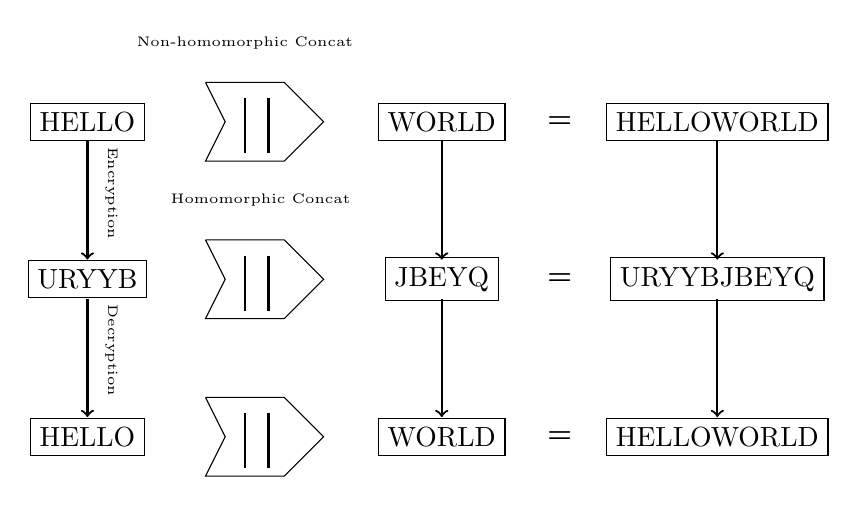
\begin{tikzpicture}

  \node[label={[label distance=0.5cm,text depth=-1ex,rotate=-90]right:\tiny Encryption}] at (1.2,5.3) {};
  \node[label={[label distance=0.5cm,text depth=-1ex,rotate=-90]right:\tiny Decryption}] at (1.2,3.3) {};


  % BOTTOM
  \node [rectangle, draw, align=center] at (1,1) {HELLO};
  \draw [thick, <-] (1,1.25) -- (1,2.75);
  \draw [thin] (2.5, 1.5) -- (3.5, 1.5) -- (4, 1) -- (3.5, 0.5) -- (2.5, 0.5) -- (2.75, 1) -- (2.5, 1.5);
 
  \draw [thick] (3, 1.3) -- (3, 0.6);
  \draw [thick] (3.3, 1.3) -- (3.3, 0.6);

  \node [rectangle, draw, align=center] at (5.5,1) {WORLD};
  \draw [thick, <-] (5.5,1.25) -- (5.5,2.75);

  \node at (7, 1) {\textbf{=}};

  \node [rectangle, draw, align=center] at (9,1) {HELLOWORLD};
  \draw [thick, <-] (9,1.25) -- (9,2.75);


  %MIDDLE
  \node [rectangle, draw, align=center] at (1,3) {URYYB};
  \draw [thick, <-] (1,3.25) -- (1,4.75);
  \draw [thin] (2.5, 3.5) -- (3.5, 3.5) -- (4, 3) -- (3.5, 2.5) -- (2.5, 2.5) -- (2.75, 3) -- (2.5, 3.5);
  \node [align=center] at (3.2, 4) {\tiny Homomorphic Concat};
  \draw [thick] (3, 3.3) -- (3, 2.6);
  \draw [thick] (3.3, 3.3) -- (3.3, 2.6);

  \node [rectangle, draw, align=center] at (5.5,3) {JBEYQ};
  \draw [thick, <-] (5.5,3.25) -- (5.5,4.75);
  \node at (7, 3) {\textbf{=}};

  \node [rectangle, draw, align=center] at (9,3) {URYYBJBEYQ};
  \draw [thick, <-] (9,3.25) -- (9,4.75);

  %TOP
  \node [rectangle, draw, align=center] at (1,5) {HELLO};
  \draw [thin] (2.5, 5.5) -- (3.5, 5.5) -- (4, 5) -- (3.5, 4.5) -- (2.5, 4.5) -- (2.75, 5) -- (2.5, 5.5);
  \node [align=center] at (3, 6) {\tiny Non-homomorphic Concat};
  \draw [thick] (3, 5.3) -- (3, 4.6);
  \draw [thick] (3.3, 5.3) -- (3.3, 4.6);

  \node [rectangle, draw, align=center] at (5.5,5) {WORLD};
  \node at (7, 5) {\textbf{=}};

  \node [rectangle, draw, align=center] at (9,5) {HELLOWORLD};

  



\end{tikzpicture}
\end{document}
